\chapter{Model based on Inertial Measurement Unit}
\label{ch:simp_mdl}
The multibody approach in the previous chapter is computationally demanding. It cannot be implemented on real time. The bottleneck in the multibody approach is the execution time of the rigid body algorithm. In this chapter the EKF is formulated with a simple dynamic model that can run on real time is discussed. The model is based on the translational acceleration and angular velocity measured by IMU. 

\section{Mathematical model of IMU}
The IMU \emph{MTi-100 \footnote{xsens technologies \url{http://www.xsens.com/en/general/mti-100-series} }} consists of accelerometer and gyroscope. It measures the acceleration and angular rate with respect to the coordinate frame of the body with which it is attached. The acceleration measured by accelerometer is \citep{bloe12}
\begin{figure}
\begin{center}
%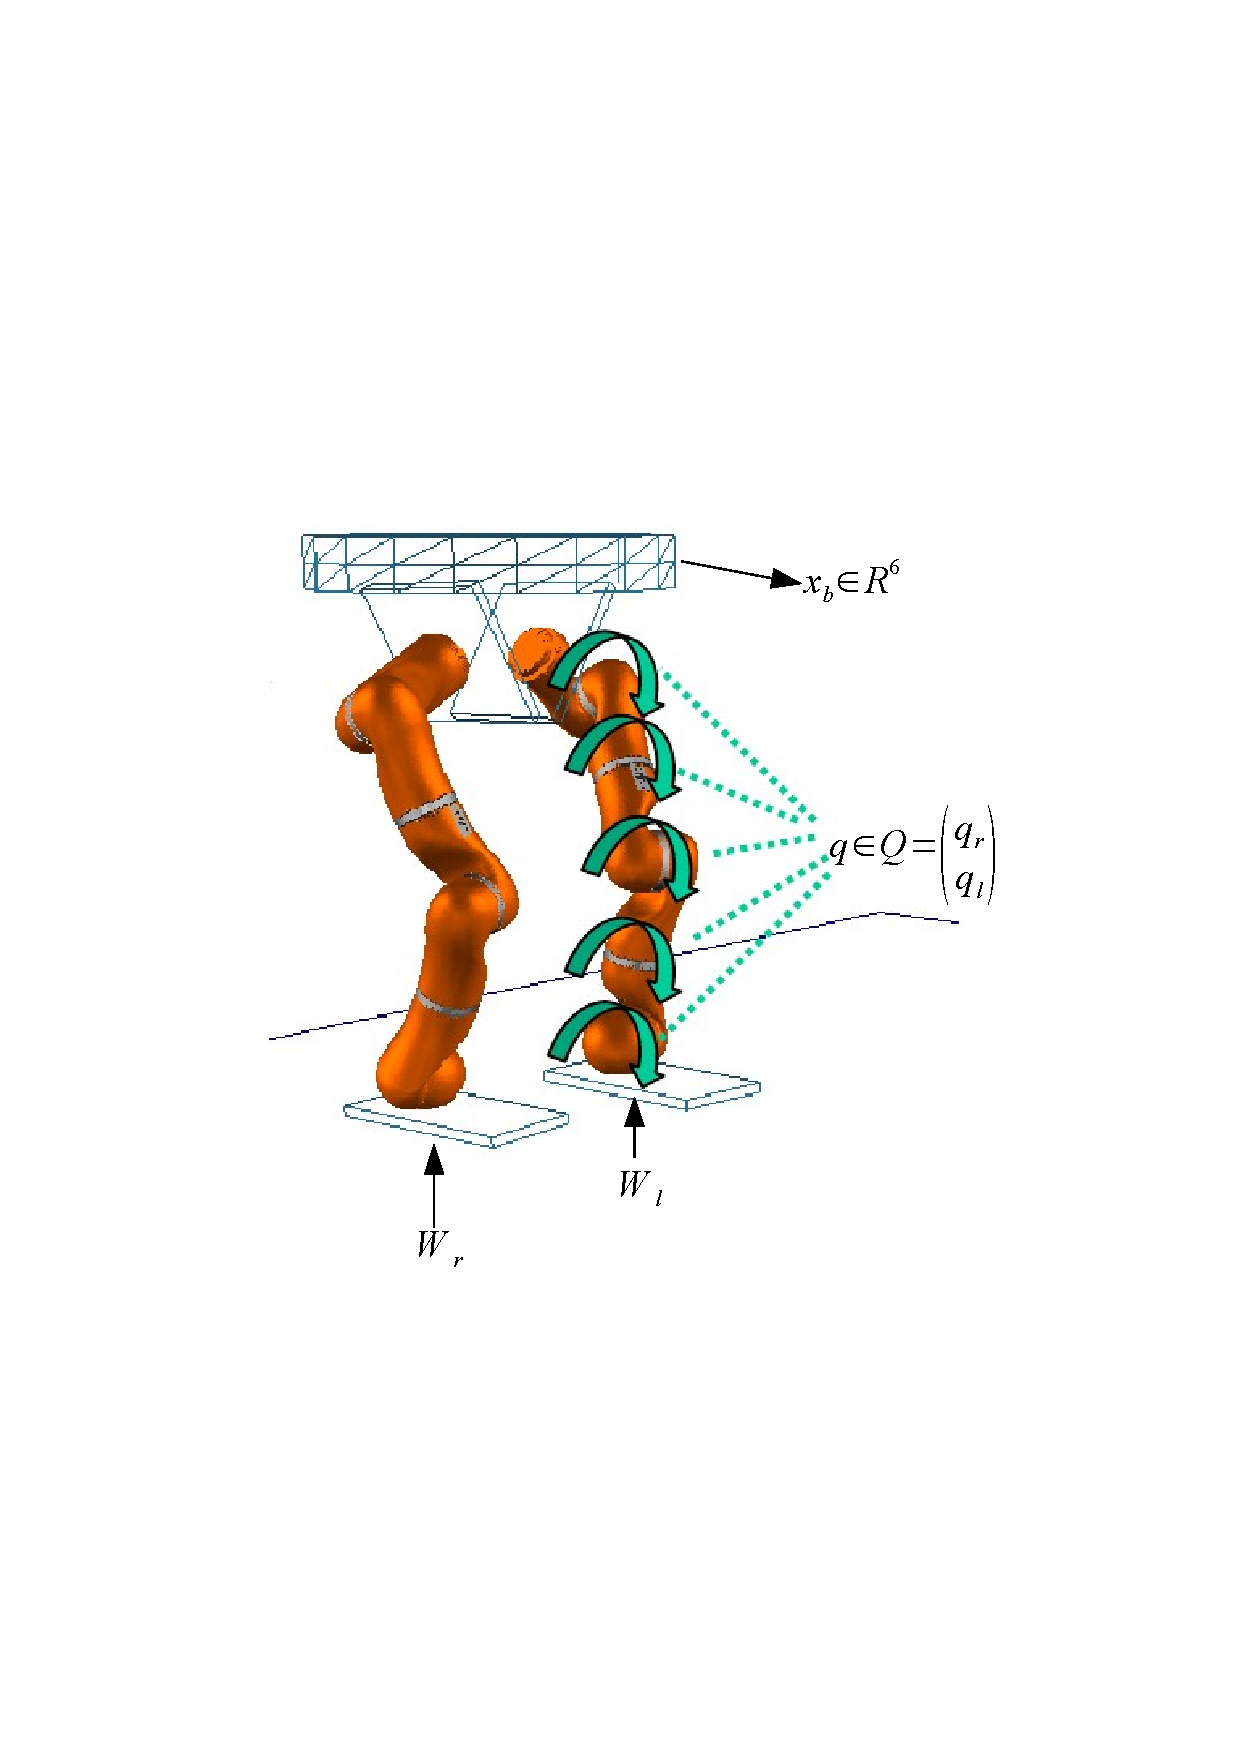
\includegraphics[trim= 10mm 80mm 10mm 80mm,scale=0.75]{Bilder/model_biped.pdf}
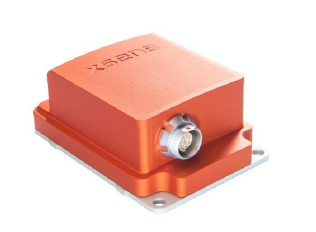
\includegraphics[scale=0.75]{Bilder/pic_imu.png}
\caption{IMU(\emph{MTi-100} mounted) on \emph{Toro}}
\label{fig:toro_imu}
\end{center}
\end{figure}
\begin{equation}
    \label{eq:imu_acc}
    a = R(a_{abs} - g),
\end{equation}
where $a_{abs} $ is the absolute acceleration of the body with respect to spatial frame (world frame) and \emph{g} denotes the acceleration due to gravity $[0,0,-9.81]^T$.

The measurement from the IMU are noisy. In addition to the noise there can be bias acting on the measurements. The stochastic model of the IMU is 
\begin{equation}
\label{eq:imu_noise}
\begin{split}
\tilde{a} &= a + b_a + w_a \\
\dot{b}_a &= w_{ba} \\
\tilde{\omega} &= \omega + b_\omega + w_\omega \\
\dot{b}_\omega &= w_{b\omega},
\end{split}
\end{equation}
where $\tilde{a}$ is the acceleration measured by the IMU. It is composed of true acceleration \emph{a}, bias $b_a$ and the sensor noise $w_a$. The measured angular velocity is $\tilde{\omega}$, true angular velocity $\omega$, bias $b_{\omega}$ and sensor noise $w_\omega$. The sensor noises $w_a$ and $w_\omega$ are modelled as zero mean Gaussian white noise. The biases $b_a$ and $b_\omega$ are dynamical quantities but they have very slow dynamics. The bias dynamics $\dot{b}_a$ and $\dot{b}_\omega$ are modelled as first order Markov process. The bias is driven by zero mean Gaussian white noises $w_{b\omega}$ and $w_{bf}$.

\subsection{State space representation}
The state space formulation of the dynamic model is based on Equation \ref{eq:fwdyn_ode}. Rearranging the Equation \ref{eq:imu_noise} in terms of true acceleration and true angular velocity and substituting Equation \ref{eq:imu_acc} in \ref{eq:imu_noise} leads to state space dynamic model: 
\begin{equation}
    \label{eq:dyn_imu}
    \begin{split}
    \dot{p} &= v \\
    \dot{v} &= a = R(\tilde{a} - b_a - w_a)+g \\
    \dot{\theta} &= T^{-1}\omega = T^{-1}(\tilde{\omega} - b_\omega - w_\omega) \\
    \dot{b}_a &= w_{ba}\\
    \dot{b}_\omega &= w_{b\omega}
    \end{split}
\end{equation}
\begin{itemize}
    \item $ p = \begin{bmatrix} p_x \\ p_y \\ p_z \end{bmatrix}$ is the position of IMU measurement frame with respect to spatial frame
    \item $ v = \begin{bmatrix} v_x \\ v_y \\ v_z \end{bmatrix} = \begin{bmatrix} \dfdx{p_x}{t} \\ \dfdx{p_y}{t} \\ \dfdx{p_z}{t} \end{bmatrix}$ is the velocity of IMU with respect to spatial frame
    \item $ \theta = \begin{bmatrix} \theta_x \\ \theta_y \\ \theta_z \end{bmatrix}$ is the orientation of the IMU frame with respect to spatial frame. The rotation matrix $R=R(\theta)$ transforms a vector in body coordinate frame to spatial coordinate frame (world coordinate frame). It is parametrized as RPY Euler angles [Appendix \ref{sec:rot_mat}]
    \item $T=T(\theta)$ is the matrix that transforms Euler rate $\dot{\theta}$ to angular velocity $\omega$ in the body coordinate frame [Appendix \ref{sec:avel_trfm}].
\end{itemize}
The states of the system are
\begin{equation}
x = \begin{bmatrix} p \\ v \\ \theta \\ b_a \\ b_{\omega} \end{bmatrix} \in \Re^{15}.
\end{equation}
The contact points in Equation \ref{eq:y_kin} are the only measurements considered in this model:
\begin{equation}
    \label{eq:y_simp}
    y = s_{cnt} = \begin{bmatrix}s_{r}\\ s_{l}\end{bmatrix},
\end{equation}
The formulation of the measurement equation is also similar to Equation \ref{eq:y_cnt}. But the homogeneous transformation of the feet $H_r$ and $H_l$ are 
$$\begin{aligned}
H_r &= H_{hip}^{s}H^{hip}_{r} \\
H_l &= H_{hip}^{s}H^{hip}_{l},
\end{aligned}$$
\begin{itemize}
    \item $H_{hip}^{s}$ is the homogeneous transformation matrix of the frame attached to the IMU and the spatial frame [Appendix \ref{sec:htm}]
    \item $H^{hip}_r$ and $H^{hip}_l$ are the transformation of foot relative to hip. It is computed by the kinematics \emph{Toro}, which is a function of joint angles \emph{q}. The joint angles are measured by joint encoders.
\end{itemize}
\paragraph{Filter switching} The contact switching in Algorithm \ref{alg:cnt_switch} should be used in this model for dealing with the line and surface contacts. The system in Equation \ref{eq:dyn_imu} is observable for surface contact but unobservable for line contact. This is due to the fact that the measurements during line contact are linearly dependent. To solve the system under these circumstances, the estimation is done only on the following states:
\begin{equation}
\label{eq:dyn_imu_red}
x=\begin{bmatrix}
p \\ v\\ \theta
\end{bmatrix} \in \Re^9.
\end{equation} The biases $b_a$ and $b_\omega$ are assumed to be constant. 

The state estimation will consist of two EKF's, one estimating the full state system in Equation \ref{eq:dyn_imu} and the other estimating the reduced state in Equation \ref{eq:dyn_imu_red}. The selection of the filter is based on the ZMP. When switching between the filters, the new filter's state $\hat{x}_0$ and covariance $P_0$ are initialized with the estimated values of old filter in previous time step. The active filter's output should be taken as the of the filter.

\begin{figure}
	\centering
	\pgfdeclarelayer{background}
\pgfdeclarelayer{foreground}
\pgfsetlayers{background,main,foreground}

% Define a few styles and constants
\tikzstyle{smallbox}=[draw, top color=white, bottom color=blue!20, text width=5em,text centered, minimum height=2.5em]
\tikzstyle{relationship} = [diamond,top color=white,bottom color=red!20,draw=red!50!black!100]
\tikzstyle{bigbox} = [smallbox,top color=white,text width=6em,fill=green!30,minimum height=5em,rounded corners]
\tikzstyle{input} = [coordinate]
\tikzstyle{sum} = [draw, fill=blue!20, circle, node distance=1cm]
\tikzstyle{output} = [coordinate]
\def\blockdist{3}
\def\edgedist{1.5}

\begin{tikzpicture}[node distance=4cm]
	\node (FTS) {FTS};
	\node (IMU)[above of=FTS,node distance=2cm] {IMU};
	\node (q) [below of=FTS,node distance=2cm,text width=3em]{Joint angles};
	\node (ZMP)[relationship,right of=FTS,node distance=3cm]{ZMP};
	\path (ZMP.north)+(0,\blockdist) node (full_trig)[input]{};
	\node (FULL)[bigbox,right of=ZMP,yshift=2cm]{Full state estimator \\ $\hat x = [\hat p,\hat v,\hat \theta,\hat b_a,\hat b_\omega]$};
	\node (FULL_Y)[right of=FULL,node distance=2cm]{$\hat x$};
	\path (ZMP.south)+(0,-\blockdist) node (red_trig)[input]{};
	\node (RED) [bigbox,right of=ZMP,yshift=-2cm]{Reduced state estimator $\hat x = [\hat p,\hat v,\hat \theta]$};
	\node (RED_Y) [right of=RED,node distance=2cm]{$\hat x$};
	\node (OUT) [output,right of=ZMP,node distance= 6.75cm]{};
	
	%\draw [->] (FTS) --node{} (ZMP.west);
	\draw [->](FTS) --node{}+(\edgedist,0);
	\draw [->](IMU) --node[above]{$a,\omega$}+(\edgedist,0);
	\draw [->](q) --node[above]{$q$}+(\edgedist,0);
	\draw [-] (ZMP) --node[right,text width=4em]{Surface contact}(full_trig);
	\draw [->] (full_trig) -|node{} (FULL.north);
	\draw [-] (FULL.east) --node{}(FULL_Y);
	\draw [-] (ZMP) --node[right,text width=4em]{Line contact} (red_trig);
	\draw [->] (red_trig) -| node{} (RED.south);
	\draw [-] (RED.east) --node{}(RED_Y);
	\draw [->] (FULL.south west)+(0.5,0) --node[left]{$\hat{x}_{k-1}, P_{k-1}$}+(0.5,-\edgedist);
	\draw [->] (RED.north east)+(-0.5,0) --node[right]{$\hat{x}_{k-1}, P_{k-1}$}+(-0.5,\edgedist);
	\draw [->] (OUT) --node[right]{}+(\edgedist,0) node[right]{$\hat x$}; 
	%Draw background layers
    \begin{pgfonlayer}{background}
        % Compute a few helper coordinates
        \path (ZMP.west |- FULL.north)+(-0.5,1.3) node (a) {};
        \path (RED.south -| FULL_Y.east)+(+0.5,-1.3) node (b) {};
        \path[fill=yellow!10,rounded corners, draw=black!50, dashed]
            (a) rectangle (b);
    \end{pgfonlayer}
\end{tikzpicture}

	\caption{Swithing model of EKF}
	\label{fig:ekf_switch}
\end{figure}

\subsection{Prediction step}
The prediction equations of EKF are given in Equation \ref{eq:ekf_predict}. 
\begin{equation}
\label{eq:imu_predict}
\begin{split}
\hat{x}_{k+1}^- &= f(\hat{x}_{k},u_{k+1},0)\\
P_{k+1}^- &= A_kP_{k}A_k^T + W_kQ_{k}W_k^T\\
\end{split}
\end{equation}
The model is discretized for the implementation of EKF. Since the time step for integration is very small $\Delta t = 1ms$ forward Euler discretization method is used to discretize the continuous time model in \ref{eq:dyn_imu}.
\begin{equation}
    \label{eq:dyn_imu_disc}
    \begin{split}
    \hat{p}_{k+1}^- &= \hat{p}_k + \Delta t \hat{v}_k + \frac{\Delta t^2}{2} (\hat{R}_k (\tilde{a}_{k+1} - \hat{b}_{a,k})+g) \\
    \hat{v}_{k+1}^- &= \hat{v}_k + \Delta t (\hat{R}_k (\tilde{a}_{k+1} - \hat{b}_{a,k})+g) \\
    \hat{\theta}_{k+1}^- &= \hat{\theta}_k + \Delta t \hat{T}_k^{-1}(\tilde{\omega}_{k+1} - \hat{b}_{\omega,k+1}) \\
    \hat{b}_{a,k+1}^- &= \hat{b}_{a,k}\\\
    \hat{b}_{\omega,k+1}^- &= \hat{b}_{\omega,k}
    \end{split}
\end{equation}
The system matrix is obtained by computing the Jacobian of the discretized system of equations is
\begin{equation}
    A_k = \begin{bmatrix}
    I_3 &\Delta t &\frac{\Delta t^2}{2} \dfdx{\hat{R}_k}{\theta}(\tilde{a}_{k+1} - \hat{b}_{a,k} ) &-\frac{\Delta t^2}{2} \hat{R}_k &\textbf{0}_3 \\
    \textbf{0}_3 &I_3  &\Delta t \dfdx{\hat{R}_k}{\theta}(\tilde{a}_{k+1} - \hat{b}_{a,k} ) &-\Delta t\hat{R}_k &\textbf{0}_3\\
    \textbf{0}_3  &\textbf{0}_3 &I_3 + \Delta t \dfdx{\hat{T}^{-1}}{\theta}(\tilde{\omega}_{k+1} - \hat{b}_{\omega,k+1}) &\textbf{0}_3 &\Delta t \hat{T}_k^{-1}\\
    \textbf{0}_3  &\textbf{0}_3  &\textbf{0}_3  &I_3 &\textbf{0}_3 \\
    \textbf{0}_3  &\textbf{0}_3  &\textbf{0}_3  &\textbf{0}_3 &I_3
    \end{bmatrix}
\end{equation}

\subsection{Update step}
The update equation of the EKF is given in Equation \ref{eq:ekf_correct}. The measurement equation of the system is given by $$\hat{y}_{k+1} = h(\hat{x}_{k+1}^-,u_{k+1},0).$$For the sake of simplicity let us assume the measurement of noise are independent. $$V_k = I_3.$$ Substituting the assumption in Equation \ref{eq:ekf_correct} leads to the following filter equations:
\begin{equation}
\label{eq:imu_correct}
\begin{split}
K_{k+1} &= P_{k+1}^-\hat{C}_{k+1}^{T}(\hat{C}_{k+1}P_{k+1}^-\hat{C}_{k+1}^{T} + R_{k+1})^{-1}\\
\hat{x}_{k+1} &= \hat{x}_{k+1}^- + K_{k+1}(y_{k+1}-\hat{y}_{k+1})\\
P_{k+1} &= (I- K_{k+1}\hat{C}_{k+1})P_{k+1}^-
\end{split}
\end{equation}

The measurement sensitivity matrix is computed by taking the Jacobian of the measurement equation.
\begin{equation}
        \hat{C}_{k+1} = \dfdx{\hat{y}_{k+1}}{x} = 
	\begin{bmatrix}		        
        \dfdx{\hat{H}^{s}_{hip,k+1}}{x} H_{hip}^r p_i\\
		\dfdx{\hat{H}^{s}_{hip,k+1}}{x} H_{hip}^l p_i\\
    \end{bmatrix}
         \hspace{1cm} \forall i=\{A,B,C,D\} 
\end{equation}
where $\dfdx{\hat{H}^s_{hip,k+1}}{x}$ is the partial derivative of homogeneous transformation matrix $H_{hip,k+1}^s$ with respect to system states. [Appendix \ref{sec:htm}]

% Experiments
\subsection{Experiment}

\begin{figure}
% We need layers to draw the block diagram
\pgfdeclarelayer{background}
\pgfdeclarelayer{foreground}
\pgfsetlayers{background,main,foreground}

% Define a few styles and constants
\tikzstyle{sensor}=[draw, fill=blue!20, text width=5em,text centered, minimum height=2.5em]
\tikzstyle{system} = [sensor, text width=6em, fill=green!30, 
    minimum height=12em, rounded corners]
\tikzstyle{input} = [coordinate]
\tikzstyle{sum} = [draw, fill=blue!20, circle, node distance=1cm]
%\tikzstyle{output} = [coordinate]
\def\blockdist{0.5}
\def\edgedist{0.75}
\begin{tikzpicture}
	% Define the nodes in the picture
	\node (sys_in)[yshift=1cm]{$x_0$};
	\node (u_in) [below of=sys_in,node distance=1cm]{$u$};
	\node (sys_u)[input,right of=u_in,node distance=1cm]{};
    \node (sim_sys) [system,right of=sys_in,node distance=3cm] {Double pendulum system};
    \node (sys_noise)[above of=sim_sys,node distance=3cm]{$n_w$};
    \node (msr_noise)[right of=sys_noise,node distance=2cm]{$n_v$};
    \node (msr_add)[sum,right of=sim_sys,node distance=2cm]{};
    \node (estimator) [system,right of=msr_add,node distance =3cm]{ Estimator};
    \node (est_in) [right of=sim_sys,node distance=3cm,yshift=1.5cm]{$\hat{x}_0$};
    \node (est_u) [input,right of =sim_sys, node distance=2cm,yshift=-3cm]{foo};
    \node (est_out)[right of=estimator,node distance=3cm]{$\hat{x}$};
    
    % Define the edges in the picture
    \draw [->] (sys_in) --node{}(sim_sys.west);
    \draw [-] (u_in) --node{}(sys_u);
    \draw [->] (sys_u) --node{}+(\edgedist,0);
    \draw [-] (sys_u) |-node{}(est_u);
    \draw [->] (est_u) |-node[pos=0.7,above]{$u$}(estimator.-130);
    \draw [->] (est_in) --node{}+(\edgedist,0);
    \draw [->] (sys_noise) --node{}(sim_sys.north);
    \draw [->] (msr_noise) --node{}(msr_add.north);
    \draw [->] (sim_sys.east) --node[above]{}(msr_add.west);
    \draw [->] (msr_add.east) --node[above]{$y$}(estimator.west);
    \draw [->] (estimator) --node{}(est_out);
\end{tikzpicture}
\caption{Experimental setup for the simple model}
\end{figure}

